% XeLaTeX style packages

\documentclass[a4paper,11pt]{article}
%\usepackage{fontspec}
%\defaultfontfeatures{Ligatures=TeX}
% \setmainfont{Liberation Serif}
\usepackage{microtype}
\frenchspacing
\usepackage{enumitem}
\usepackage{color}
\usepackage{geometry}
\usepackage{graphicx}
\usepackage{booktabs}
\usepackage{multirow}
\usepackage{hyperref}
\usepackage[backend=bibtex,sorting=none]{biblatex}
\bibliography{refs}

\begin{document}
\title{DUNE-SP Timing System: Protocol}
\begin{center}
{\LARGE\bf DUNE-SP Timing System: Protocol}
\vspace{1cm}

J. Brooke, D. Cussans, D. Newbold, S. Trilov, \\
\vspace*{1ex}
v5 -- 23rd March 2020
\end{center}
\vspace*{\fill}
\setcounter{tocdepth}{1}
\tableofcontents
\vspace*{\fill}

\section*{Summary}

This document acts as the repository for:
\begin{itemize}
\item The definition of interfaces at hardware, firmware and software level between the timing system and the other components of ProtoDUNE-SP
\item The definition of the internal protocol and assignments of command encodings, etc.
\end{itemize}
It is intended to be updated periodically as the specification is finalised and amended.

\newpage
\section{Overview}

The timing system is required to: provide a stable and phase-aligned
master clock to all DAQ components; receive external signals (including triggers)
into the ProtoDUNE clock domain and time-stamp them; distribute synchronization,
trigger and calibration commands to the DAQ system; and conduct continuous
checks of its own function. In addition, the timing system acts as a
data source, providing a record of timing signals received, distributed, or
throttled. The system is designed to meet the full eventual requirements
of the DUNE experiment, but will need only a subset of that functionality
for ProtoDUNE.

An FPGA-based master unit receives a high-quality clock (provided in
ProtoDUNE by a GPS-disciplined oscillator) and external signals from the
trigger system and SPS accelerator. It interfaces to the ProtoDUNE control
and DAQ via a gigabit Ethernet interface. The master unit multiplexes
synchronization and trigger commands, along with arbitrary command
sequences generated by software, into a single encoded data stream,
which is broadcast to all timing endpoints, and decoded into separate clock
and data signals. A uniform phase-aligned cycle counter, updating at the
ProtoDUNE system frequency of 50MHz, is maintained at all endpoints,
allowing commands to take effect simultaneously at all endpoints
regardless of cable lengths or other phase delays.

The timing signal is broadcast via multi-mode optical fiber, with conversion to
LVDS signals over short twisted pair cable for backwards compatibility with existing
timing interfaces (e.g. on SSPs). The system uses duplex links, allowing all endpoints
to be regularly interrogated during system operation to verify correct operation
and reception of timing commands. Along with the possibility to select
any given endpoint via a unique network address, this mechanism also allows
automatic phase-adjustment of all local clocks at system start-up,
through precise measurement of the returned clock phase at the master unit. The definition
of timing groups allows the system to be partitioned into a number of
independent timing zones.

Endpoints decode the timing signal into separate clock and data
signals using a commercial clock-data-recovery device, which in turn
can feeds a low-bandwidth PLL for applications requiring a very low jitter local clock.
The data stream employs 8b/10b encoding, ensuring sufficient transitions in the
timing signal for clock recovery and correct operation of optical links, and uses a random idle 
pattern to minimise EMI from copper segments. A common firmware block is used to
decode the timing protocol, which is incorporated into the overall
firmware design for the receiving FPGA in each DAQ component. This
block provides a cycle counter, several independent trigger, calibration and 
synchronisation signals, and a general-purpose packet data output to each endpoint.
The cycle counter may be used further to generate low-frequency timing signals for
further propagation, e.g. the 2MHz sampling signal for the cold ADCs.

\begin{figure}[p]
	\centering
	\includegraphics[angle=90,height=0.9\textheight]{figs/timing.pdf}
	\caption{Simplified system overview}
	\label{fig:timing}
\end{figure}

\section{Timing Master Interfaces}

\subsection{Timing Master Functions}

The timing system operates in a master-slave configuration. All timing signals are broadcast by the master, and interpreted by slaves. Responses from slaves are only generated when requested by the master.

The timing master has the following functions:

\begin{itemize}
	\item Reception of master clock signal and serialised time-of-day information (e.g. from an external GPS receiver)
	\item Reception of external timing and trigger signals
	\item Logging and time-stamping of signals received, distributed or throttled, and transmission to DAQ
	\item Serialisation of timing commands and transmission to the timing network
	\item Phase measurement of incoming timing signals from slaves, allowing phase adjustment under software control
	\item Transmission of arbitrary commands and control data under software control
\end{itemize}

\subsection{Timing Master Implementation}

The master unit is physically implemented as a pair of custom FMC cards, hosted by an FPGA-based carrier module. The interface FMC (based on the AIDA mini-TLU~\cite{TLU}) receives external signals from the trigger, SPS accelerator interface, and other external sources, and provides a number of spare general-purpose IO interfaces. The timing FMC, which is also used elsewhere in the timing system, provides clock-data recovery and jitter reduction functions and the serial optical interface to the timing system.

\subsection{Master Clock Interface}

The master unit receives a clock frequency reference from an external source (e.g. GPS-disciplined oscillator or White Rabbit clock distribution system). In the absence of an external source, including under laboratory conditions, the system clock may be produced internally from a programme quartz oscillator source. For ProtoDUNE-SP, the clock frequency is fixed at 50.0MHz, dictated by the requirements of the TPC front end electronics.

In addition, the master unit can receive a synchronized serial data stream from an external source for external timestamping of events. The master unit is able to output the system clock or a divided version of it for monitoring or other purposes.

\subsection{Trigger Inputs}

The master unit receives trigger information via an serial link, using the same protocol as for general timing information. Since the timing master and trigger processor are expected to be adjacent, this link is implemented using LVDS signals.

The master unit receives up to six external trigger inputs via single-ended coaxial connectors (LEMO 00). These inputs feed discriminators, and may be used as edge or level sensitive inputs for the trigger distribution logic. On arrival, signals are registered into the ProtoDUNE-SP timing domain, and the receipt of signals is recorded and available to DAQ. Since external signals not aligned with the system clock must be re-registered, it is not guaranteed that signals that are synchronous in the driving clock domain will be registered on the same 50MHz cycle.

\subsection{Other External Inputs}

Non-trigger external inputs may be received synchronized into the ProtoDUNE-SP timing domain, and used either as stimulus for automatic synchronous commands, or gates or vetos for any trigger signal. An example of such a signal is the SPS spill warning signal.

\subsection{Run Control and DAQ Interface}

The master unit interfaces to the ProtoDUNE-SP computing system for run control and DAQ, via a gigabit Ethernet interface. The system uses the IPbus protocol for all communication. Functions available to software include:

\begin{itemize}
	\item Timing system reset and configuration
	\item Measurement of endpoint clock phases
	\item Enabling and disabling of automatic synchronous commands (i.e. those issued in response to trigger inputs)
	\item Configuration of periodic synchronous commands (e.g. for calibration)
	\item Issuing of asynchronous commands
	\item Readout of buffered trigger information
\end{itemize}

{\color{red}FUTURE\_UPDATE} Full specification of registers, etc, should be documented here.

\section{Timing Protocol and Transport}

\subsection{Timing Signal Functions}

The 50MHz clock and timing commands are distributed to all timing endpoints as a broadcast signal. However, synchronous commands may be addressed to specific timing groups, and asynchronous commands may be addressed to individual endpoints or timing groups.

\subsection{Timing Signal Implementation}

Conversion between the transport methods defined below will be handled by an conversion module, implemented by the timing FMC card. Conversion takes place transparently at protocol level. The FMC card also acts as a test platform for protocol development, and as a reference design for the timing interface of ProtoDUNE-SP DAQ modules. A top-level diagram of the FMC signal paths is shown in Figure~\ref{fig:FMC}.

\begin{figure}[p]
	\centering
	\includegraphics[angle=90,height=0.9\textheight]{figs/FMC.pdf}
	\caption{Timing FMC signal paths}
	\label{fig:FMC}
\end{figure}

\subsection{Layer 0: Physical Signalling}

Clock and data are typically distributed as a single signal, using a CDR device at endpoints to recover separate clock and data signals. However, some endpoints may need to be supplied with a separate clock signal, and this is supported via the timing FMC.

The data stream is encoded as a 100Mb/s DC-balanced signal suitable for distribution via optical or electrical interfaces. This low data rate allows the use of inexpensive components designed for 100Mb/s ethernet: either 100base-SX fibre optics, or Cat5/6 twisted pair cable with RJ45 connectors. 

There are three defined transport methods for the timing signal:

\begin{enumerate}
	\item Encoded data stream transported via optical fibre. The optical interface is implemented via commercial plug-in SFP modules, allowing flexibility in implementation. It is anticipated for ProtoDUNE-SP that 100base-SX components will be used, i.e. using simplex multimode fibre at 850nm wavelength for up to 500m transmission distance. Division and recombination of signals will be via passive commercial splitter modules (for lab use), with inactive endpoints disabling their optical transmitter, or via an active fan out (for use at the experiment site with large numbers of endpoints).
	\item Encoded data stream transported via LVDS over twisted pair. Two pairs will carry broadcast and return data respectively. Division of signals will be via an active fan-out unit if required (e.g. as implemented on the WIB crate backplane), recombination of signals will be via an active logical 'or' or Bus LVDS wire-or, with inactive endpoints transmitting continuous '0' level. This method is expected to be used on crate backplanes only.
	\item Encoded data stream along with a separate phase-aligned clock signal, transported via LVDS over twisted pair. A third pair will be used to carry the clock signal. Returned data is transmitted on the same clock. This method will be used only for point-to-point signalling, for compatibility with existing interfaces.
\end{enumerate}

Conversion between these three methods is transparent at protocol level, with the same encoded data stream used regardless of whether an explicit clock signal is transmitted.

\subsection{Layer 1: Data Link}

The data stream uses 8b/10b encoding to transmit one byte per five 50MHz clock cycles. The standard comma mechanism is used for word alignment, with K28.5 used as the comma character. The timing data stream consists of a sequence of synchronous packets, asynchronous packets, and idle packets, in that order of priority.

\begin{itemize}
	\item Synchronous packets begin with a K28.1 character (/S/), and are of fixed two-character length. Synchronous packets may interrupt other traffic at any time, and carry synchronous commands that are guaranteed to be issued at endpoints in the correct order, and with a fixed timing relationship to their request at the master unit.
	\item Asynchronous packets are of arbitrary length, begin immediately on the first non-comma character encountered in the data stream, and end with a K28.5 character (/C/). Asynchronous packets carry general control information to endpoints, that is not guaranteed to arrive with a fixed latency.
	\item Idle packets are a particular type of asynchronous packet, transmitted when no other packet information is queued. They consist of a pseudorandom byte sequence in order to minimise EMI due to repetitive patterns during link idle. Idle packets are of short length to ensure sufficient comma density for rapid link alignment.
\end{itemize}

Return data uses the same protocol, with the exception that endpoints never send synchronous commands. Figure~\ref{fig:wave} shows an simplified example of the structure of the timing data stream. Note that, in practice, a minimum period of ~1ms of idle packets is required after an endpoint is requested to send data, in order for the optical link amplifiers to stabilise and master unit CDR chip to lock.

\begin{figure}[p]
	\centering
	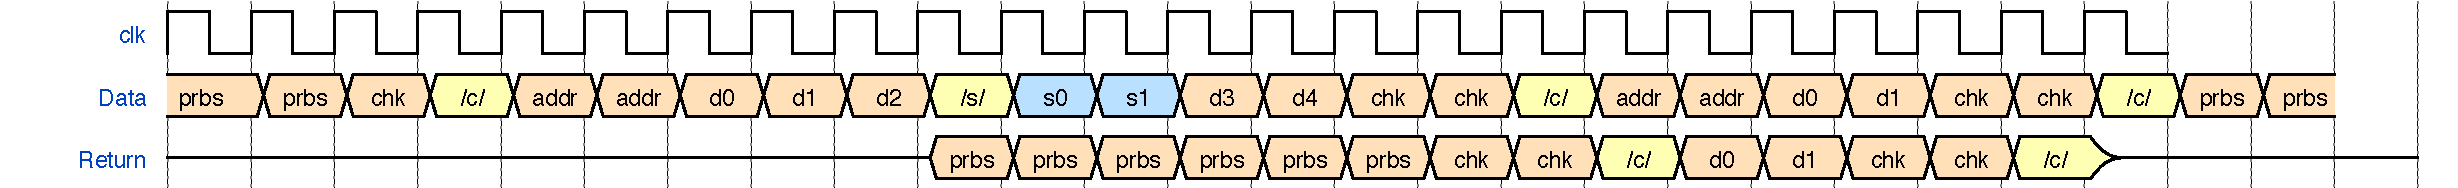
\includegraphics[width=0.9\textwidth]{timing_protocol_wavedrom_01.pdf}
	\caption{Example timing data stream}
	\label{fig:wave}
\end{figure}

\subsection{Layer 2: Addressing and Protocol}

The synchronous and asynchronous packet formats are shown in Tables~\ref{tab:async} and \ref{tab:sync}.

\begin{table}[h!]
  \centering
  \begin{tabular}{@{}ll@{}} \toprule
    Byte & Content \\ \midrule
    0 & /S/ (K28.1) \\
    1 & Group / Command \\ \bottomrule
  \end{tabular}
  \caption{Synchronous packet format}
  \label{tab:sync}
\end{table}

\begin{table}[h!]
  \centering
  \begin{tabular}{@{}ll@{}} \toprule
    Byte & Content \\ \midrule
    0 & Address(7:0) \\
    1 & Address(15:8) \\
    2 & Command \\
    3 & Data byte 0 \\ 
    $3 + n$ & Data byte $n$ \\ 
    $3 + n + 1$ & Checksum(7:0) \\
    $3 + n + 2$ & Checksum(15:8) \\
    $3 + n + 3$ & /C/ (K28.5) \\ \bottomrule
  \end{tabular}
  \caption{Asynchronous packet format}
  \label{tab:async}
\end{table}

Synchronous packets contain a single four-bit timing group specifier, and a single four-bit command. The command field encodes sixteen separate synchronous commands, corresponding directly to the sync outputs of the decoder block. Every timing endpoint may be configured with a timing group mask, such that it accept synchronous commands addressed only to selected timing groups. This allows flexible partitioning of the system.

The timing protocol allows transmission of synchronous commands at a rate of no more than once per 10 clock cycles, which is adequate for the low rate of synchronous commands expected in both ProtoDUNE-SP and DUNE. In the event of clashing synchronous commands, a priority encoding scheme is used, such that lower-numbered commands pre-empt high-numbered ones, and lower-numbered timing groups pre-empt higher numbered ones. Under rare or pathological conditions this may result in a synchronous command being rejected; a record is kept of all propagated and rejected signals.

Asynchronous packets contain a single one-byte command followed by an arbitrary number of data bytes. The address is a unique experiment-wide 16b endpoint identifier, or has the special value of 0xfff in the top 12 bits for a broadcast packet, with the timing group identifier in the bottom four bits. The checksum is a standard CRC-16-CCITT, calculated on all packet bytes including the address. Return data packets lack the address field, but are otherwise identical. Idle packets are identified by the all-zeroes address, and contain random data which is not interpreted further by the endpoint, except to validate the checksum.

{\color{red}FUTURE\_UPDATE} Document the ProtoDUNE-SP address assignment.

\subsection{Layer 3: Command assignment}

Currently defined synchronous and asynchronous commands are shown in Tables~\ref{tab:sync_cmds}, \ref{tab:async_cmds} and \ref{tab:async_ret_cmds}. In the case of synchronous command queue conflict, priority for transmission is assigned to lower-numbered commands (i.e. counter sync command has priority over all over traffic). Asynchronous commands meant to be interpreted internally by the timing system endpoint decoder use are distinguished by a 0 in the topmost bit of the command byte.

\begin{table}[h!]
  \centering
  \begin{tabular}{@{}llp{9cm}@{}} \toprule
    Cmd bit & Name & Notes\\ \midrule
    0 & S\_Sync & Used to align and check system cycle counter; issued at 1ms intervals \\
    14 & S\_Spill & SPS spill warning toggle \\
    15 & S\_Trig & Beam trigger signal \\ \bottomrule
  \end{tabular}
  \caption{Synchronous commands}
  \label{tab:sync_cmds}
\end{table}

\begin{table}[h!]
  \centering
  \begin{tabular}{@{}lllp{9cm}@{}} \toprule
    Cmd & Name & Data bytes & Notes\\ \midrule
    0x0 & A\_Reset & 0 & Resets state of endpoint \\
    0x1 & A\_Sync & 8 & Stores cycle counter value to be loaded at next S\_Sync \\
    0x2 & A\_Enable & 0 & Enables endpoint transmission \\
    0x3 & A\_Status & 1 & Request endpoint status packet transmission \\ 
    0x4 & A\_Adjust & 2 & Adjusts packet delay and clock phase of endpoint \\ \bottomrule
  \end{tabular}
  \caption{Asynchronous commands}
  \label{tab:async_cmds}
\end{table}

\begin{table}[h!]
  \centering
  \begin{tabular}{@{}lllp{9cm}@{}} \toprule
    Cmd & Name & Data bytes & Notes\\ \midrule
    0x0 & R\_Status & TBD & Endpoint status report \\ \bottomrule
  \end{tabular}
  \caption{Asynchronous return commands}
  \label{tab:async_ret_cmds}
\end{table}

{\color{red}FUTURE\_UPDATE} Define further synchronous and asynchronous commands.

\section{Timing Endpoint Interfaces}

\subsection{Timing Endpoint Functions}

A timing endpoint is characterised by the following properties:

\begin{itemize}
	\item A single system clock phase, adjustable under timing system control
	\item A unique address
	\item A timing group mask
\end{itemize}

A conceptual diagram of an endpoint is shown in Figure~\ref{fig:fw_if}. It consists of three major components:

\begin{itemize}
	\item A clock and data recovery IC (e.g. ADN2814). This component is not required for endpoints with a clock + data interface.
	\item A PLL for jitter reduction and phase adjustment, with the latter function controlled from the endpoint FPGA. The PLL may be implemented as an internal clock controller (e.g. MMCM) within the FPGA, or may be an external component. This component is not required for endpoints with a clock + data interface, since phase may be controlled by the optical-LVDS converter module if necessary.
	\item A firmware protocol decoder, implemented inside the FPGA as part of the overall system firmware. This block receives and interprets the timing data stream, and provides decoded commands to other blocks inside the FPGA. It also monitors and counts errors observed in the data stream.
\end{itemize}

Error conditions monitored by the decoder include:

\begin{itemize}
	\item 8b/10b decoder errors
	\item Packet checksum errors
	\item Counter-out-of-sync error
	\item CDR / PLL lock timeout
\end{itemize}

The status of the decoder may be monitored locally via the status flags (see below), or for soft errors, remotely via the R\_Status command. An endpoint that is in error can be reset locally or via the timing system, and then brought back into synchronisation with the rest of the system at the next S\_Sync command.

\begin{figure}[p]
	\centering
	\includegraphics[width=0.9\textwidth]{figs/fw_if.pdf}
	\caption{Endpoint signal paths}
	\label{fig:fw_if}
\end{figure}

\subsection{Endpoint Firmware Interface}

The decoder block exposes three sets of signals:

\subsubsection{sys\_clk domain signals}

\begin{itemize}
	\item {\bf sys\_clk} (o) is the free-running local clock provided by the host FPGA
	\item {\bf sys\_rst} (i) is a startup synchronous reset signal
	\item {\bf address} (i) is a 32b word specifying: the address identifying this endpoint (see above for addressing scheme); and the timing group mask. It should not change once sys\_rst is released.
	\item {\bf status} (o, 4b) is a set of output signals indicating the internal state of the decoder, including: whether the core is in contact with the timing master; is in one of several possible setup or error conditions; is providing a stable global clock. The signal may be used to drive a reset of all logic governed by the global clock.
\end{itemize}

{\color{red}FUTURE\_UPDATE} Write state transition diagram for the decoder.

\subsubsection{Global\_clk domain signals}

\begin{itemize}
	\item {\bf global\_clk} (i) is the phase-adjusted 50MHz system clock from the PLL
	\item {\bf sync} (o, 16b) is a set of bits corresponding to decoded synchronous command content. These bits go high for one clock cycle on receipt of the corresponding synchronous command.
	\item {\bf cmd} (o, 8b) is a byte-wide output carrying a copy of received packet data addressed to this endpoint.
	\item {\bf strobe} (o) is a signal qualifying the validity of the cmd output. It stays high for an entire packet of data, then goes low at the end of the packet.
	\item {\bf timestamp} (o, 64b) is the 64b system cycle counter, cycling at global clock frequency.
\end{itemize}

\subsubsection{Other signals}

\begin{itemize}
	\item {\bf data} (i) is the recovered or received serial timing data stream. This signal is automatically registered on the rising or falling edge of global\_clk in order to cope with arbitrary phase alignment.
	\item {\bf cdr\_lock} (i) is the lock status signal of the CDR chip
	\item {\bf pll\_lock} (i) is the lock status of the PLL
	\item {\bf pll\_adj} (i, 8b) is a word indicating the desired phase adjustment for global\_clock. The physical interface to the PLL is implemented by the host FPGA, since this may require communication via a range of means to the PLL depending on implementation.
\end{itemize}

\section{System Level Operations}

The steps required to accomplish basic system level operations are listed below in simplified form. These steps are driven by software.

{\color{red}FUTURE\_UPDATE} Add calibration sequences as required.

\subsection{System Startup}

This procedure is carried out at system startup.

\begin{enumerate}
	\item Reset and initialise timing master unit
	\item Perform master self-test via timing path loopback
	\item Enable command transmission
\end{enumerate}

\subsection{Phase Adjustment}

This procedure is carried out after endpoints are powered and reset, but before final endpoint initialisation. It is assumed that a 'running' status from the timing decoder will be a necessary step in individual endpoint initialisation sequences. For each endpoint in turn, phase adjustment is carried out as follows:

\begin{enumerate}
	\item Enable endpoint transmission
	\item Wait for CDR lock and measure clock phase
	\item Request status packet
	\item Measure whole-cycle offset to establish path delay to / from endpoint
	\item Issue delay / phase adjustment command
	\item Verify correct alignment
	\item Disable endpoint transmission
\end{enumerate}

This process is estimated to require around 10ms per endpoint (dominated by the time required for CDR lock and clock phase measurement), allowing ProtoDUNE-SP to be brought up in a few seconds.

{\color{red}FUTURE\_UPDATE} Document measured phase adjustment time as measured in hardware.

\subsection{Operations Startup}

This procedure is carried out after all endpoints are aligned, and after time-of-day is established via GPS.

\begin{enumerate}
	\item Reset master cycle counter
	\item Enable command and input logging
	\item Enable regular S\_Sync commands
	\item Enable trigger commands
\end{enumerate}

\subsection{System Monitoring}

System monitoring is continually carried out by continuous repetition of the endpoint phase check sequence, and logging of any error counts reported by endpoints. This activity has lower priority than other system activities.

\subsection{Operations Shutdown}

This procedure is carried out after all DAQ queues have drained, as one of the last end-of-run steps.

\begin{enumerate} 
	\item Disable trigger commands
	\item Wait until next S\_Sync command
	\item Disable regular S\_Sync commands
	\item Issue S\_Reset
	\item Disable command and input logging
\end{enumerate}

\section{ProtoDUNE-SP Interfaces}

\subsection{Clock source interface}

The master unit will receive a 10MHz clock signal and IRIG time-of-day data from a local White Rabbit timing distribution unit, which is responsible for forwarding signals from the SPS control room. This approach ensures synchronization with the ProtoDUNE beam instrumentation, which has a separate timing system, but based on the same clock.

\subsection{Trigger interface}

The trigger processor will be a client of the timing system, in that it will receive clock and command data via the (LVDS version of) the standard timing interface. Unlike other endpoints, however, the trigger processor is permitted to send synchronous commands on the return path, which carry trigger information. This mechanism allows the transmission of up to 14 different trigger types.

\subsection{WIB interface}

The WIB crate PTC will receive an optical signal from the timing system, convert this to a serial electrical signal, and distribute to the WIBs themselves via the backplane. At protocol level, each WIB constitutes a timing system endpoint. The WIB will contain a stand-alone jitter-reducing PLL for clock forwarding to the TPC front end electronics. 

\subsection{COB interface}

The COB will receive fibre from the timing system, via the RTM. The RTM will distribute timing signals to the DTM, which will constitute the timing endpoint. Internal clock and timing signals will then be distributed to the RCEs. The COB will implement a PLL internally to the DTM FPGA.

\subsection{FELIX interface}

There will be no hardware interface to FELIX. The timing system control software will send trigger messages to FELIX over the network, including timestamp information.  It will also be necessary to send any signal that results in a reset of timestamp counters.

\subsection{SSP interface}

The SSP will receive the three-signal timing interface (clk, din, dout) via an optical-LVDS converter module.

\subsection{CRT interface}

The muon veto readout system will receive a a clock and simple synchronisation pulse from the timing system, generated by a timing FMC acting as a self-contained endpoint.

\clearpage
\printbibliography

\end{document}
